\begin{figure}[h!]
    \centering 
    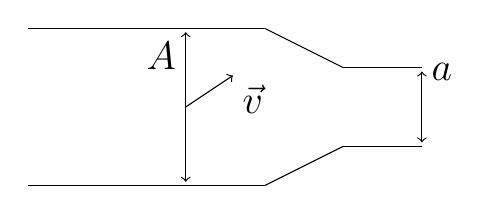
\begin{tikzpicture}
        \draw 
            (-2,1)--(1,1);
        \draw 
            (-2,-1)--(1,-1);
        \draw 
            [<->, black] (0,-0.95)--(0,0.95) node[anchor= north east]{\Large $A$};
        \draw 
            [->, black] (0,0)--(0.6, 0.4) node[anchor= north west]{\Large$\vec{v}$};
        \draw 
            (1,1)--(2,0.5);
        \draw 
            (1,-1)--(2,-0.5);
        \draw 
            (2,0.5)--(3,0.5);
        \draw 
            (2,-0.5)--(3,-0.5);
        \draw 
            [<->, black] (3,-0.45)--(3,0.45) node[anchor= west]{\Large$a$};
    \end{tikzpicture}
    \caption{Schematic depiction of the De Lavalle nozzle.}
    \label{fig:nozzle}
\end{figure}